\chapter{Empirical Work}\label{ch:4}

We now employ empirical tests to bring some of the theories outlined in previous chapters to the Australian data. We first describe our data, derived from the Survey of Income and Housing, a periodic sample survey conducted by the ABS between 1981 and 2012, and the O*NET database of occupational tasks.

The first theory we test is the standard `canonical' model of SBTC. Second, we test a slightly more nuanced version of this model, which makes provisions for three types of labor. Finally, we test whether a Roy-type model of changes in the occupational wage structure can be explained by the task content of occupations.

We require data on real wages, as well as detailed measures of the tasks performed by participants of each occupation. For this analysis, we obtained microdata for the Survey of Income and Housing (SIH) for 1981/82, 2000/01 and 2011/12, as well as measures contained in the O*NET database, published by the US Department of Labor. Details of both the task measures and SIH are discussed in detail in the data appendix (\S\ref{sec:SIH}, \S\ref{sec:onet}). We shall therefore only briefly review the salient features of the data sources as they relate to this analysis.\footnote{There are a variety of data sources available. For a discussion of our choice of the SIH, please see the appendix.}

\section{Testing the Canonical Model}\label{sec:testsbtc}

As we have seen, the `canonical model' of SBTC explains the increase in observed inequality as a rise in the premium that accrues to high-skilled workers (\S\ref{sec:canonical}). To review, the argument for an increasing skill premium, observed in the US and UK, is that advances in technology have led to an excess of demand over supply for college-educated workers \citep{Katz1992}.

\subsection{Data}

The Survey of Income and Housing is a hierarchical clustered household survey conducted by the ABS every 2-3 years since 1995, and also for the fiscal years 1985/86 and 1981/82. The survey provides detailed  information about respondents' labor and non-labor income sources, as well as data on age, educational attainment, hours worked, industry and occupation. For the surveys conducted between 2000 and 2010, as well as the 1981-2 survey, the data include detailed occupational codes, which will become important later. The other surveys include occupation only at the one-digit level. We obtain survey micro-data as confidentialized unit record files (CURFs).

We treat the multiple surveys as repeated cross-sectional measures of the working population. In this study, we are interested in the changing value of `skills', not in individuals' wealth {\em per se}: some care needs to be taken to ensure that comparisions are consistent. Following \citet{Acemoglu2011} and others, we consider only full-time workers, and `composition adjust' the workforce according to age, sex and educational attainment to ensure that any differences in incomes are not due to mechanical, demographic changes in the composition of the work force. We include only those individuals whose incomes are received as employee wages, or as the proceeds from unincorporated entities, including the value of entitlements, tips and bonuses. Revenue from government payments, investment dividends, and so on, are ignored. Nominal incomes are deflated using the CPI, averaged over the four quarters of the survey's fiscal year.

\subsection{Results}

If SBTC explained the widening of the income distribution, then we would expect to observe the premium accruing to `skilled' labor increasing with time. In the United States, such an increase was indeed observed. There, the wage premium earned by tertiary-educated labor fell in the 1970s, but has risen each decade since then \citep{Acemoglu2011}. \citet{Katz1992} employ a similar empirical model which explains the rise of the skill premium in the United States in the post-war era. In Australia, however, a corresponding growth in the premium for tertiary qualifications has not been observed. Figure~\ref{fig:wagepremium} shows the log skill premium for Australia and the United States between 1981/82 and 2008.

\begin{figure}
  \centering
  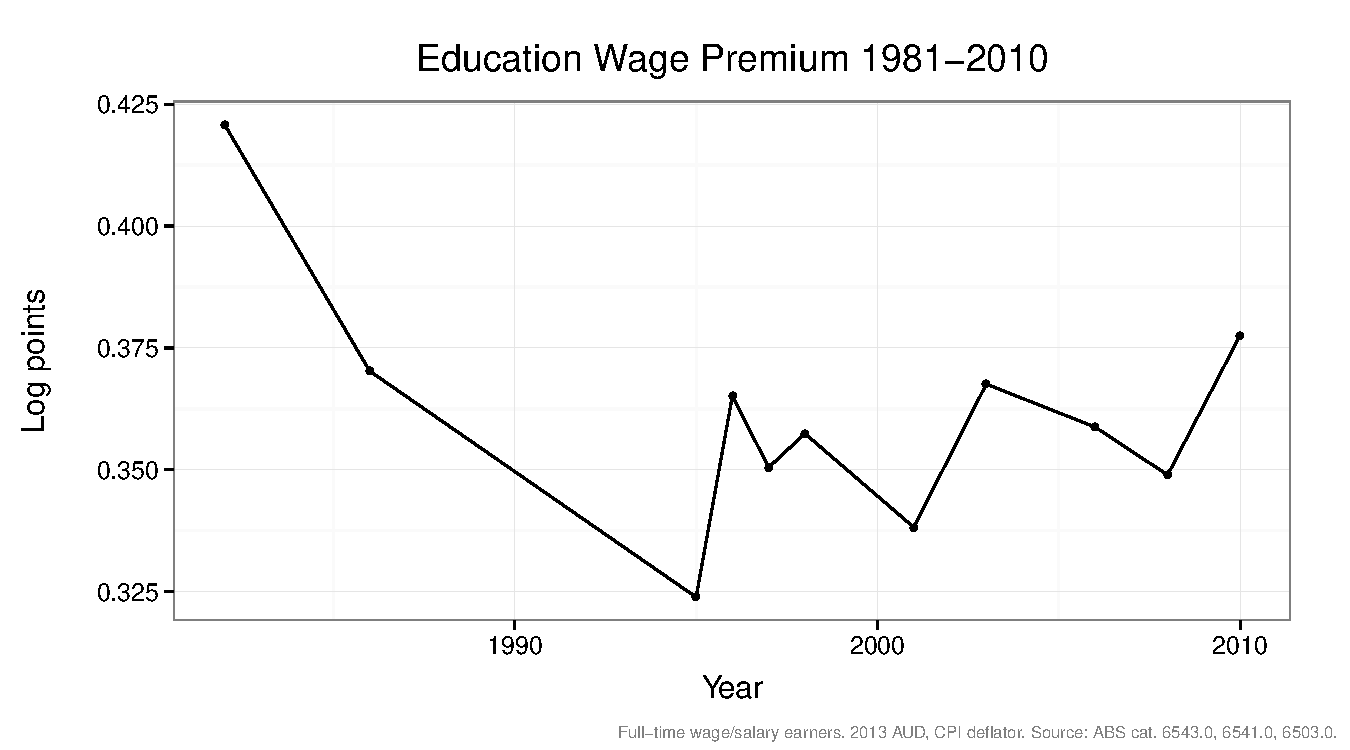
\includegraphics[width=\textwidth]{../figure/ed_premium_time_two.pdf}
  \caption{University/non-university log wage premium, Australia and the United States. The figure shows the difference between the mean log weekly income for workers who have attained a bachelor degree or higher, and the mean log weekly income of other workers. Only full-time workers whose main sources of income are wages and salaries are included, and survey data have been composition adjusted for sex, age group, (and for the United States, race). Source: for Australia, ABS Survey of Income and Housing, and for the United States, \citet{Acemoglu2011}.}
  \label{fig:wagepremium}
\end{figure}

However, the absence of a rising wage premium does not provide sufficient evidence to invalidate the model. Recall that the growth of the wage premium is explained not simply as a function of the high/low technology ratio, but also of the relative supply and demand ratios of low- and high-skilled workers. Recall that, in the \citet{Katz1992} implementation of the model given by \eqref{eq:regcanonical}, the log wage premuium is a function of both the technology ratio $(A_H/A_L)$ and the ratio of labor employed $(H/L)$. Other authors have concluded that a similar technology trend is present in the Australian data, but that the expanding supply of skilled workers has grown in lock-step with demand, leading to no increase in the skill premium.

The canonical model implies that real wages will never decrease for either skilled or unskilled workers \citep{Acemoglu2011}. This gives rise to two falsifiable predictions: first, that wage growth should be increasing with skills, because higher-skilled individuals should experience greater wage growth than lower-skilled individuals. Second, wage growth should be monotonic over time. Since technology is assumed to be continually increasing, and is also assumed to be purely skill-augmenting, there is no provision in the theory for a decrease in absolute wages.

\begin{figure}
  \centering
  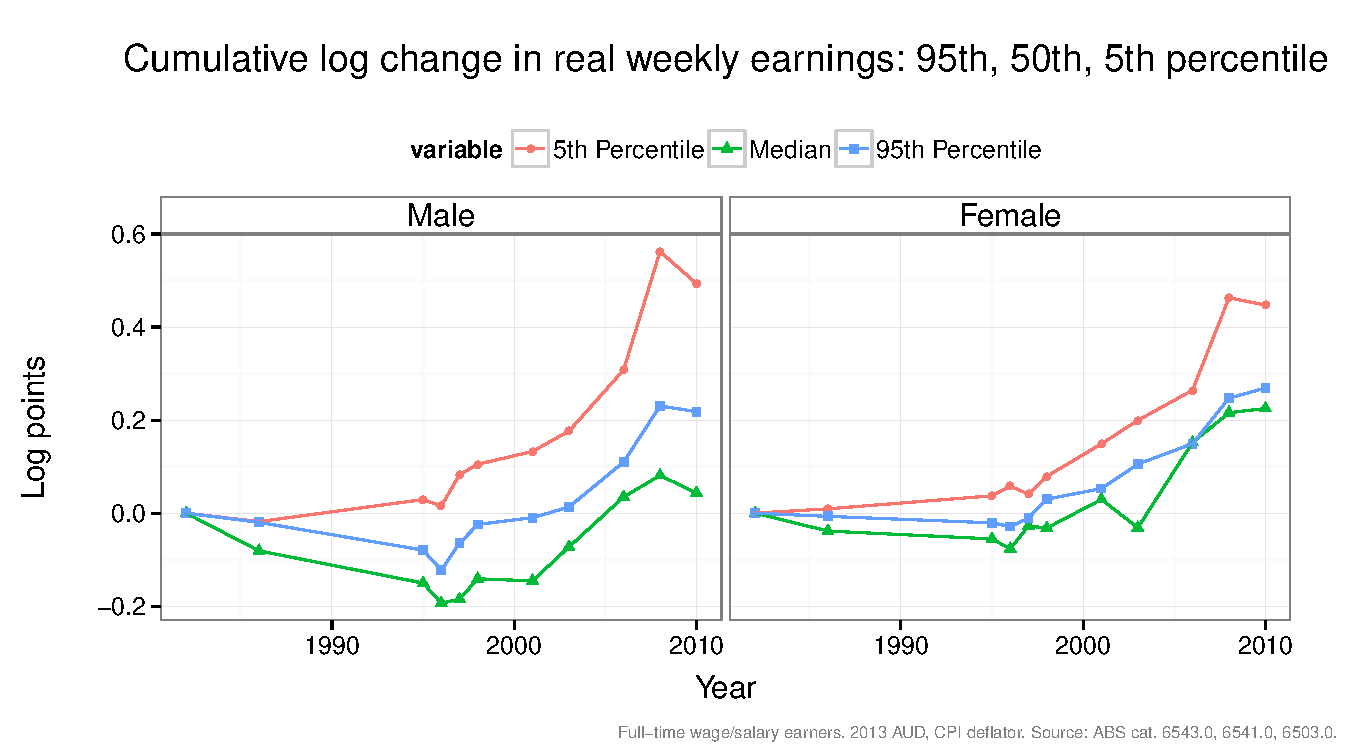
\includegraphics[width=\textwidth]{../figure/wage_change_time.pdf}
  \caption{Cumulative log change in real weekly earnings, 5th, 50th and 95th percentiles, 1982-2010. Full-time workers whose main sources of income are wages and salaries are shown. Notice that real wage growth has been non-monotonic for males in lower percentiles. Source: Survey of Income and Housing.}
  \label{fig:changetime}
\end{figure}

Figure~\ref{fig:changetime} plots the cumulative change over time for three wage percentiles, the 5th, 95th, and the median. Over the period 1981-82 to 2009-10, although wages at the top percentiles increased steadily, the same is not true for the lower percentiles. Indeed, for all of the 1990s and much of the 2000s, cumulative real income growth from 1981-82 was negative for many workers. At best, this suggests that technological change does not explain all of the observed changes in the wage distribution.

With the data we have available, we are unable to directly observe skill or individuals from period to period. We are thus unable to test the assertion that wages should be rising in the level of skill. However, \citet{Goos2007} and \citet{Acemoglu2011}, who also only have repeated cross-sectional data available, overcome this problem by treating wage percentile as a proxy for skill levels.  Figure~\ref{fig:banana} shows the composition-adjusted changes in log real wage by percentile, for males and females, between 1981-82 and 2009-10. If the 1981-82 income percentile can be considered a proxy for skill, then it is apparent that, over this period, wages grew for high-skilled individuals much faster than for low-skilled individuals. For males, wage growth is monotonic, as predicted by the model: those further up the income distribution (i.e. presumed to have higher skill levels), experienced greater wage growth. However, note that, for females, percentile wage growth is non-monotonic; the lower income quantiles experienced greater wage growth than the median.

\begin{figure}
  \centering
  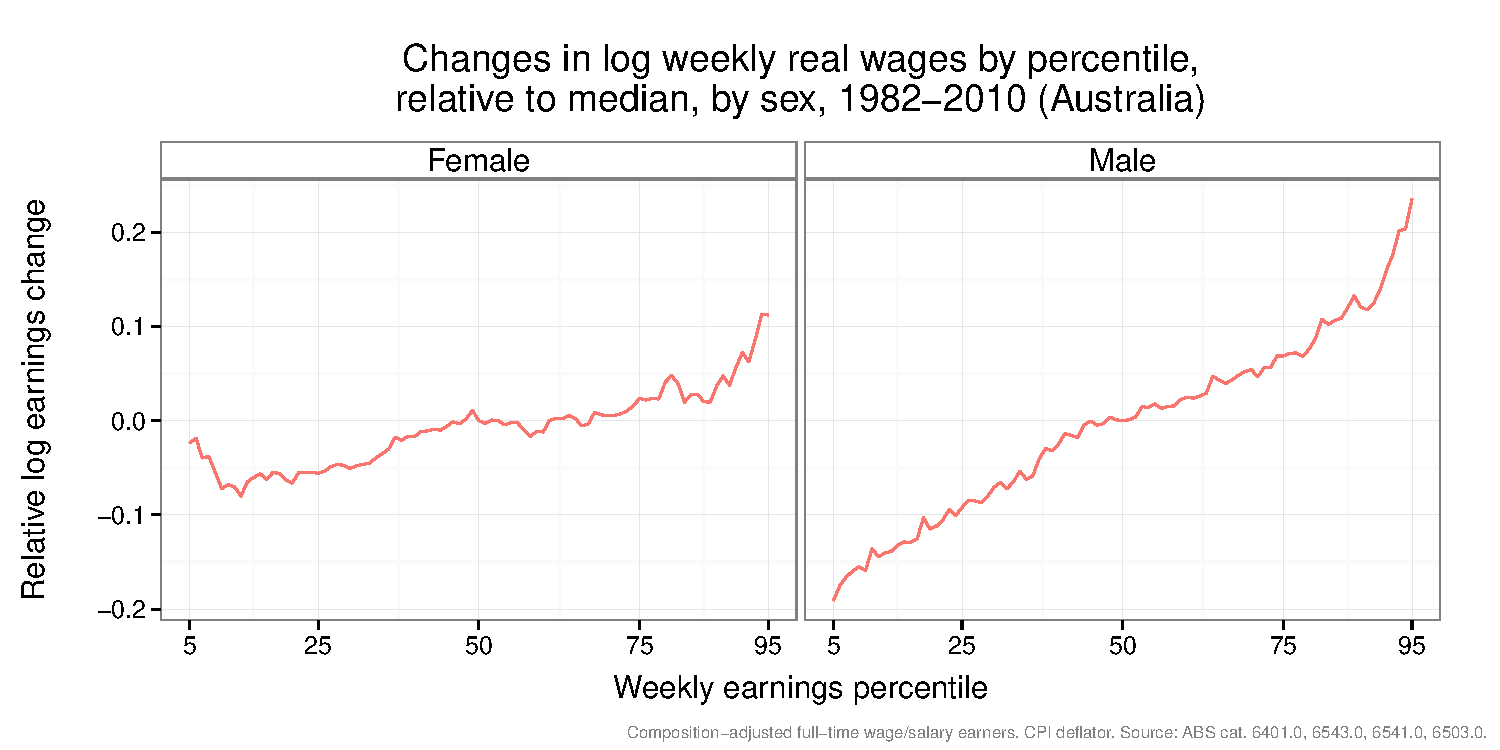
\includegraphics[width=\textwidth]{../figure/quantile_mf.pdf}
  \caption{Change in weekly wage by percentile, 1981/82--2009/10, Males and Females. Full-time workers whose main sources of income are wages and salaries are shown. Notice that real wage growth has been non-monotone for females in lower percentiles. Source: Survey of Income and Housing.}
  \label{fig:banana}
\end{figure}

\subsection{Discussion}

The evidence discussed in this section is only partially in agreement with the canonical model of SBTC laid out in Chapter~\ref{ch:2}. The model predicts an increase in inequality, as agents invest in education and increase the gap between `skilled' and `unskilled' workers. This trend is indeed observed (Figure~\ref{fig:ineq}). However, in the model, the channel through which income inequality increases is the college premium. This is not the case in Australia (Figure~\ref{fig:wagepremium}). Further regularities in the data speak against the model: non-monotonicity in wage quantiles and wages over time suggest that the SBTC story may not be the most helpful explanation.

That the income distribution is widening, but the skill premium is {\em not} driving the change, suggests at least two interpretations. We have already discussed the fact that educational attainment may be a poor indicator of skill for the Australian labor market. A second, more nuanced explanation was suggested by \citet{Levy2003}. Technological change may not be complementary to all types of labor; it may in fact be a {\em substitute} for certain jobs.

\section{The `Disappearing Middle'}\label{sec:disappearing}

The previous section suggests that, in Australia, the relationship between technology and wages are not as simple as the canonical model suggests. Evidence in the empirical literature suggests that it is middle-skilled jobs, rather than simply low-skilled jobs, that are fading from the work force over time \citep[e.g.][]{Harding1997,Cully1999,Esposto2012}. We do not attempt to replicate the existing empirical literature here; evidence for slow growth in middle-skill jobs up to 2006 were demonstrated by \citet{Esposto2012}. However, for the purposes of this investigation, we will refine the SBTC model employed above (\S\ref{sec:testsbtc}) to include a more nuanced understanding of `skill,' following the division suggested by \citet{Levy2003}.

\subsection{Model}

To test this pattern for Australian data, we can augment \eqref{eq:prod} by introducing a third type of labor, $M$, to represent work which requires mid-level skill and low levels of physical activity, representing `routine' or `middling' work. We also introduce computer capital, $C$, as a substitute in production for medium-skilled labor, and a complement in production for high-skilled workers.

First, as with the canonical model, suppose a competitive economy is governed by an CES aggregate production function which employs three types of workers: low-skilled, medium-skilled, and high-skilled. We do not necessarily require that workers of each type are homogeneous or earn the same wage. We do, however, assume that the wage, per efficiency unit, for each type of labor is fixed. As before, we call the sets of high-, medium- and low-skilled workers $\EH$, $\M$, and $\ELL$, respectively. Then we can define the aggregate inputs of each worker type by summing over the inputs of each worker $i$, measured in efficiency units: ${H = \int_{i\in\EH}h_i\;di}$, ${M = \int_{i\in\M}m_i\;di}$, and ${L = \int_{i\in\ELL}\ell_i\;di}$.

Crucially, the aggregate production function also depends on ICT capital, $C$, which is a complement in production for high-skilled workers, and a substitute for medium-skilled workers. Then, the production function is given by,
\begin{equation}  \label{eq:prod2}
Y = \left[
  \left(A_LL \right)^\frac{\sigma-1}{\sigma}
  +
  \left(A_MM + C\right)^\frac{\sigma-1}{\sigma}
  +
  \left((A_HH)^\mu + C^\mu\right)^\frac{\sigma-1}{\mu\sigma}
  \right]^\frac{1}{\sigma-1}.
\end{equation}
\citet{Michaels2010} use a formulation similar to \eqref{eq:prod2} to show that, if ICT investment $C$ increases exogenously, the wage share for high-skill workers should increase, but decrease for low-skill workers. Likewise, the wage premium for high-skilled workers should rise with increasing ICT investment, and fall for medium-skilled workers.\footnote{Following \citet{Michaels2010}, we focus on the wage {\em share}, and not the absolute wage. Although wages for high-skilled and low-skilled workers should increase with increased investment, the comparative static predictions for medium-skilled workers are indeterminate. Michaels et al. prove that the comparative static predictions for the wage share, however, are unambiguous.} To test these predictions, \citet{Michaels2010} specify a simple linear functional form to test the impact of ICT investment on the wage share for type of labor $S\in\{H,M,L\}$, estimated for broad industry groups across eleven countries, using educational attainment as a proxy for skill. The authors find support for the claim that ICT investment is associated with a decrease in the demand for middle-skilled labor. 

Adapting their specification for Australia gives the empirical model shown below. In this model, $SHARE^S$, computed as ${\sum_k W^S_k/\sum_{s,j}W^s_j}$, is the wage bill share for the labor category $S$, $C$ is ICT capital, $K$ is non-ICT capital, and $Q_i$ is value added by industry $i$. 
\begin{equation} \label{eq:translog}
\Delta SHARE^S = \alpha_{CS}\log(C/Q)_{it} + \alpha_{KS}\log(K/Q)_{it} + \alpha_{QS}\log(Q)_{it} + \epsilon_{it}.
\end{equation}
As Michaels {\it et al.} point out, the polarization hypothesis is consistent with coefficient estimates where $(\alpha_{CM}<0)$ and $(\alpha_{CH}>0)$.

\subsection{Data}

With the results from the previous section in mind, to adapt this specification for Australia requires an alternative yard-stick for `skill.' Following \citet{Levy2003}, we perform a simple, subjective partitioning of occupations according to the tasks they involve, as described by the ANZSCO major groups. For the purposes of this very simple and informal model, we divide occupations into three categories: `non-routine manual' (low-skilled, $L$), `routine' (middle-skilled, $M$), and `non-routine cognitive' (high-skilled, $H$). To deal with differences in occupational coding, we use the ANZSCO--ASCO II link table provided by the ABS (Table~\ref{tbl:link}).

Capital series were derived from national accounting data. Our data include measures of ICT capital, collected by the ABS as part of the National Accounts. For this study, we consider the aggregate ICT capital series, as well as two components: {\em software}, and {\em electrical and electronic equipment}. {\em Software} includes both commercial off-the-shelf packages, as well as custom-built line-of-business programs, whereas the second variable includes telecommunications equipment and other electronic machinery. To smooth out variation in the data, the  period 1996-2010 was divided into two seven-year periods.

\subsection{Results}

The results from estimating \eqref{eq:translog}, given in Table~\ref{tbl:sharereg}, lend mixed support for the polarization hypothesis. While estimates for $\alpha_{MS}<0$ and $\alpha_{HS}>0$ have the expected sign, they are not significant when estimated with all the parameters specified in $\eqref{eq:translog}$. However, with just electrical and electronic equipment included in regression, $\alpha_{MS}$ is negative and significant at the 5\% level. Column (4) of Table~\ref{tbl:sharereg} suggests that, over a seven-year period, a 10\% increase in electrical and electronic equipment capital is associated with a decrease in the wage share of middle-skilled workers of around 0.2, whereas it is associated with a relative increase in the wage share of high-skill workers versus low-skilled workers.

The sign of coefficient estimates for the {\em software} variable are opposite to that of {\em equipment}. This suggests a qualitative difference between software capital and equipment capital: perhaps it is a complement to medium-skilled labor? It is certainly the case that many middle-skilled occupations, such as call-center clerks, make heavy use of software capital; this is one possible avenue for future research. Since {\em equipment} includes telecommunications infrastructure, one interpretation is that {\em outsourcing}, rather than a direct application of labor-saving capital, is responsible for the decline in middle-skill labor.

\begin{figure}
  \centering
  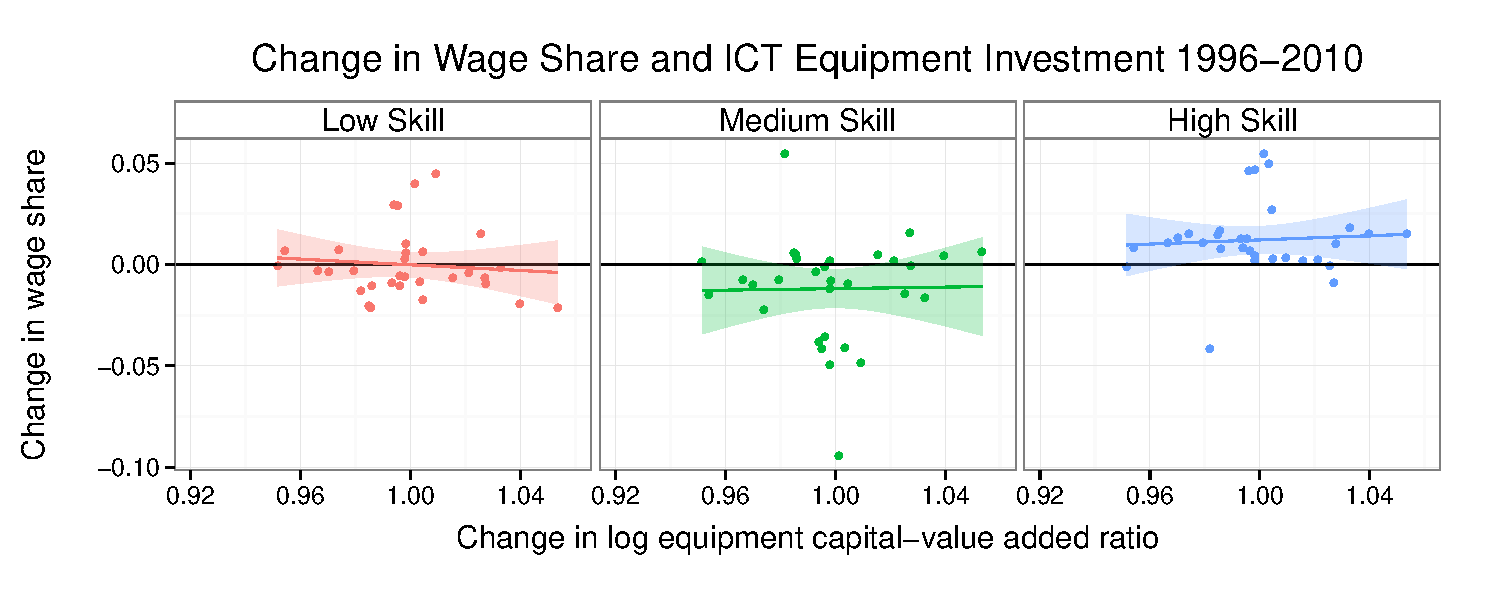
\includegraphics[width=\textwidth]{../figure/wage_share_ict.pdf}
  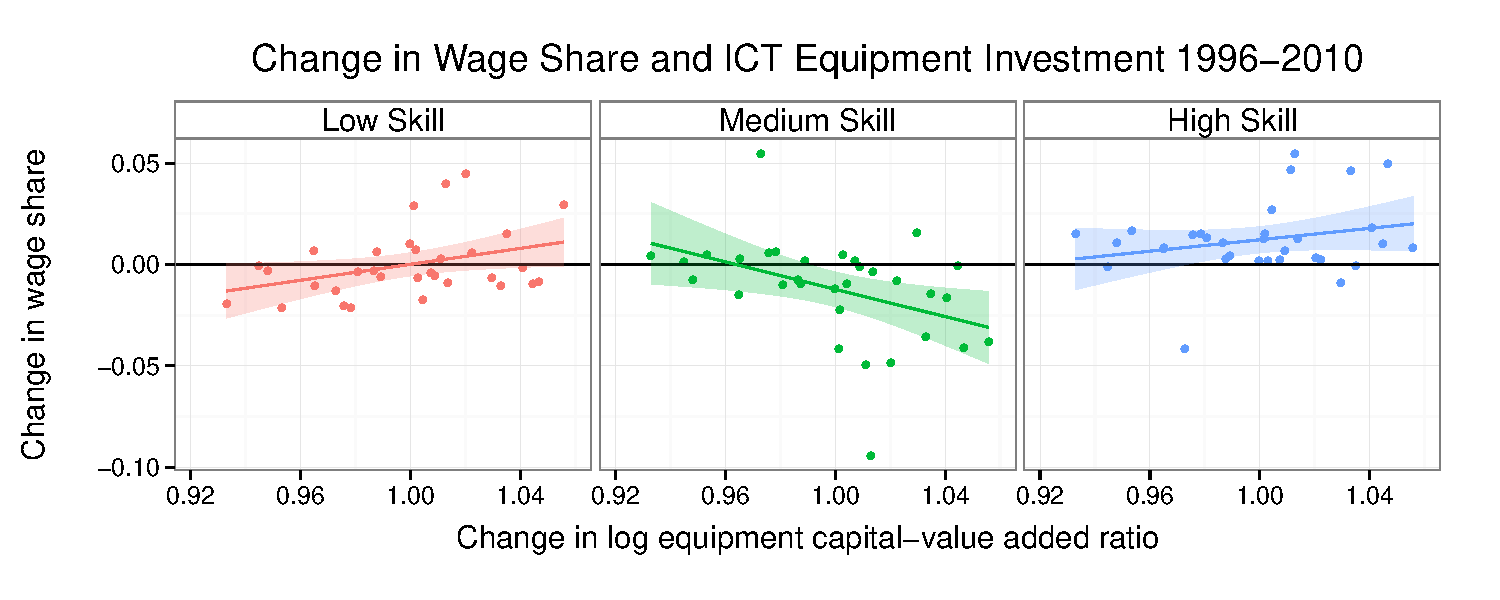
\includegraphics[width=\textwidth]{../figure/wage_share_equipment_skill.pdf}
  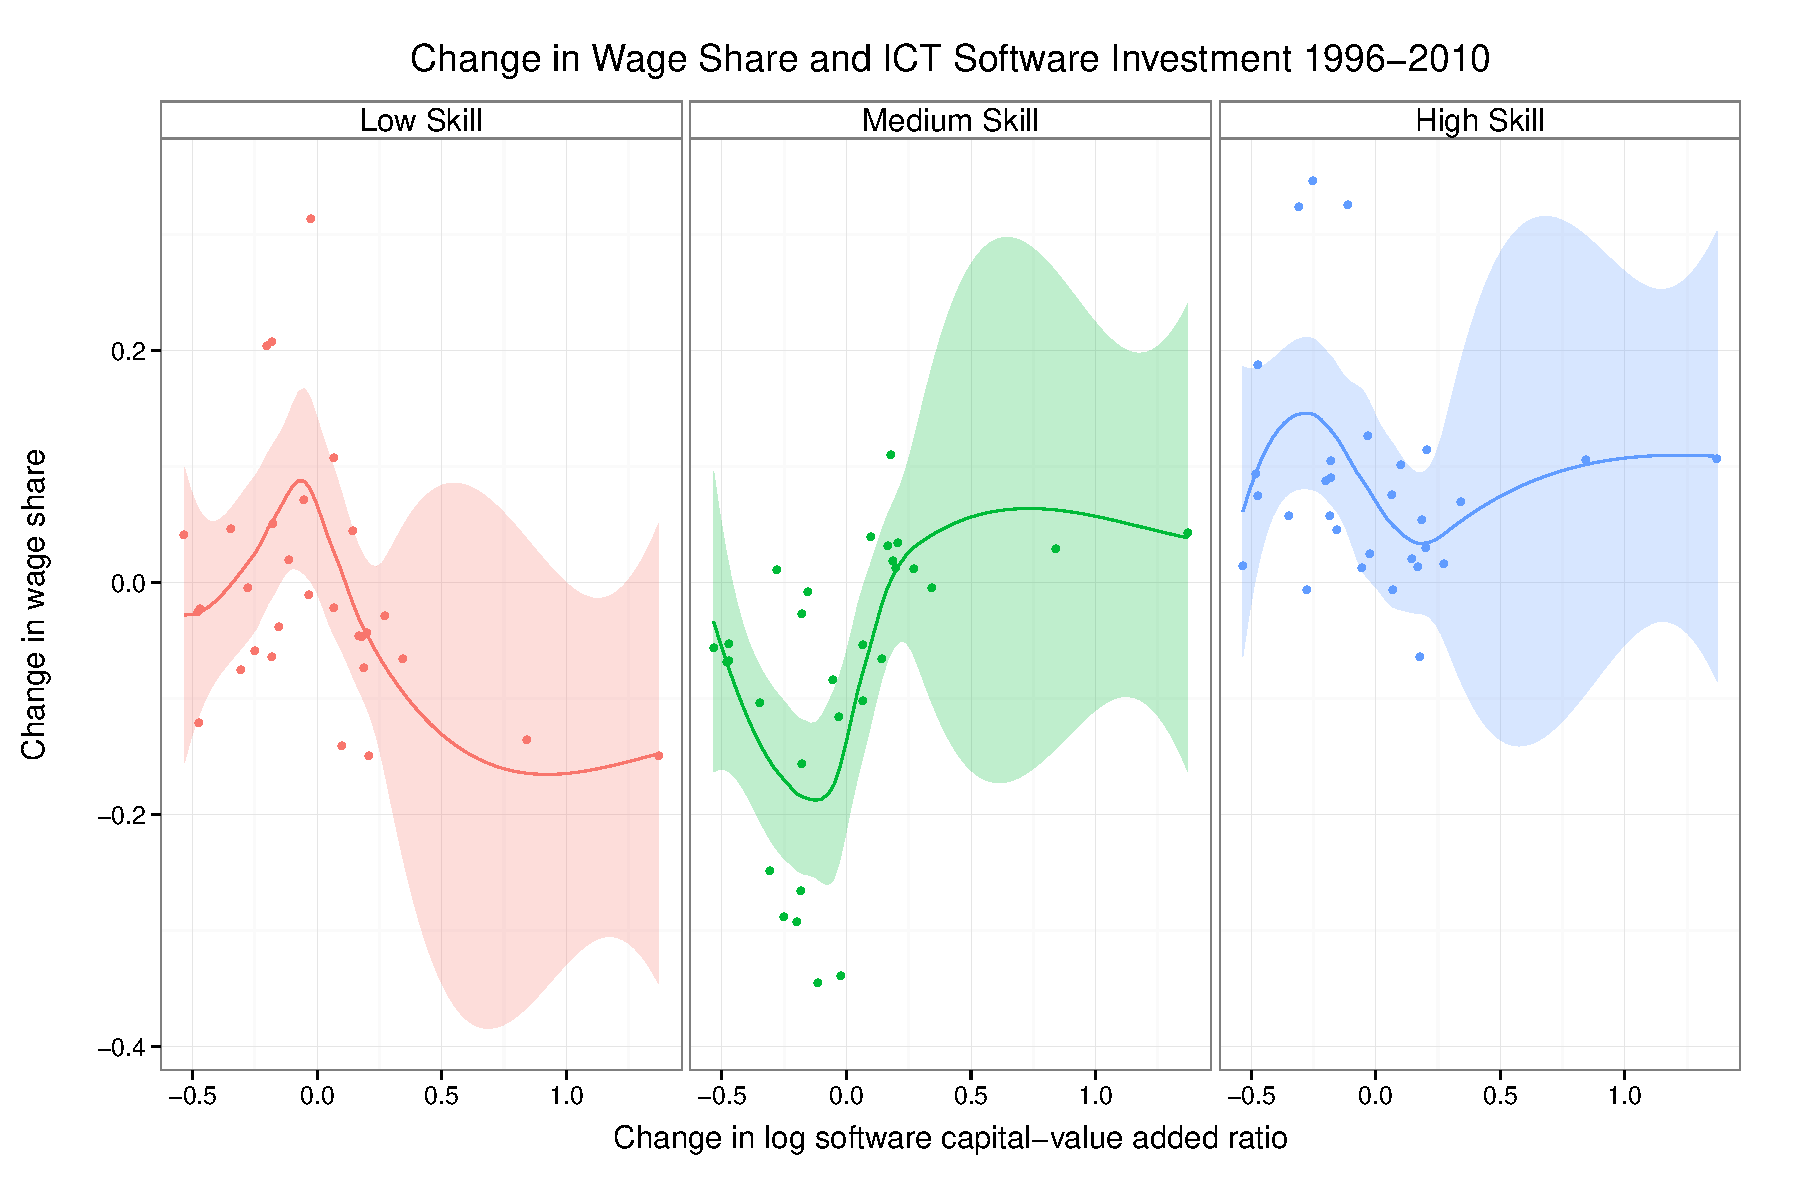
\includegraphics[width=\textwidth]{../figure/wage_share_software_skill.pdf}
  \caption{Change in wage share against change in: (1) change in log overall ICT capital ratio, (2) change in log ICT electrical and electronic equipment capital ratio, (3) change in log ICT software capital ratio, by industry, Australia, 1996-2010.
    Fitted line computed using OLS regression with ordinary 95\% confidence interval. See note for Table~\ref{tbl:sharereg} for further details. Source: ABS (Survey of Income and Housing and National Accounts).
  }
  \label{fig:equip}
\end{figure}

\begin{sidewaystable}
{\footnotesize


% Table created by stargazer v.4.0 by Marek Hlavac, Harvard University. E-mail: hlavac at fas.harvard.edu
% Date and time: Mon, Nov 04, 2013 - 13:11:20
\begin{tabular}{@{\extracolsep{0.5pt}}lD{.}{.}{-3} D{.}{.}{-3} D{.}{.}{-3} D{.}{.}{-3} D{.}{.}{-3} D{.}{.}{-3} D{.}{.}{-3} D{.}{.}{-3} D{.}{.}{-3} } 
\\[-1.8ex]\hline 
\hline \\[-1.8ex] 
 & \multicolumn{9}{c}{\textit{Dependent variable:}} \\ 
\cline{2-10} 
\\[-1.8ex] & \multicolumn{3}{c}{$\Delta SHARE^H$} & \multicolumn{3}{c}{$\Delta SHARE^M$} & \multicolumn{3}{c}{$\Delta SHARE^L$} \\ 
\\[-1.8ex] & \multicolumn{1}{c}{(1)} & \multicolumn{1}{c}{(2)} & \multicolumn{1}{c}{(3)} & \multicolumn{1}{c}{(4)} & \multicolumn{1}{c}{(5)} & \multicolumn{1}{c}{(6)} & \multicolumn{1}{c}{(7)} & \multicolumn{1}{c}{(8)} & \multicolumn{1}{c}{(9)}\\ 
\hline \\[-1.8ex] 
 $\Delta$ {\em ICT capital} & 0.045 &  &  & 0.102 &  &  & -0.147 &  &  \\ 
  & (0.147) &  &  & (0.198) &  &  & (0.127) &  &  \\ 
  & & & & & & & & & \\ 
 $\Delta$ {\em Non-ICT capital} & 0.236 &  &  & -0.546^{*} &  &  & 0.310 &  &  \\ 
  & (0.190) &  &  & (0.256) &  &  & (0.163) &  &  \\ 
  & & & & & & & & & \\ 
 $\Delta$ {\em equipment} &  & 0.143 &  &  & -0.335^{*} &  &  & 0.191^{*} &  \\ 
  &  & (0.103) &  &  & (0.136) &  &  & (0.089) &  \\ 
  & & & & & & & & & \\ 
 $\Delta$ {\em software} &  &  & -0.049 &  &  & 0.174^{*} &  &  & -0.125^{*} \\ 
  &  &  & (0.059) &  &  & (0.078) &  &  & (0.048) \\ 
  & & & & & & & & & \\ 
 $\Delta$ {\em value added} & 0.178 & 0.064 & 0.030 & -0.131 & 0.081 & 0.190 & -0.047 & -0.145 & -0.220 \\ 
  & (0.172) & (0.142) & (0.147) & (0.232) & (0.187) & (0.193) & (0.148) & (0.122) & (0.120) \\ 
  & & & & & & & & & \\ 
\hline \\[-1.8ex] 
Observations & \multicolumn{1}{c}{32} & \multicolumn{1}{c}{32} & \multicolumn{1}{c}{32} & \multicolumn{1}{c}{32} & \multicolumn{1}{c}{32} & \multicolumn{1}{c}{32} & \multicolumn{1}{c}{32} & \multicolumn{1}{c}{32} & \multicolumn{1}{c}{32} \\ 
R$^{2}$ & \multicolumn{1}{c}{0.063} & \multicolumn{1}{c}{0.067} & \multicolumn{1}{c}{0.028} & \multicolumn{1}{c}{0.149} & \multicolumn{1}{c}{0.179} & \multicolumn{1}{c}{0.155} & \multicolumn{1}{c}{0.179} & \multicolumn{1}{c}{0.179} & \multicolumn{1}{c}{0.227} \\ 
Adjusted R$^{2}$ & \multicolumn{1}{c}{-0.037} & \multicolumn{1}{c}{0.002} & \multicolumn{1}{c}{-0.039} & \multicolumn{1}{c}{0.058} & \multicolumn{1}{c}{0.122} & \multicolumn{1}{c}{0.097} & \multicolumn{1}{c}{0.091} & \multicolumn{1}{c}{0.123} & \multicolumn{1}{c}{0.174} \\ 
\hline 
\hline \\[-1.8ex] 
\textit{Note:}  & \multicolumn{9}{r}{*p $<$ 0.05; **p $<$ 0.01} \\ 
\normalsize 
\end{tabular} 


}
\caption{{\em Wage shares computed for full-time workers, whose primary sources of income are wages and salaries, estimated for 16 industry groups. `High skill' workers include professionals and managers, `middle skill' workers include sales persons, clerical workers and para-professionals, and `low skill' workers include jobs with a high degree of manual activity, including laborers, transport workers and trades persons. To smooth out noise, all variables are estimated in seven-year differences. Survey data are composition adjusted by age bracket, sex and education level to be consistent with 2010 demographics. The variables {\em equipment} and {\em software} respectively refer to the capital stock of electronic and electrical equipment and computer software, at the end of each period. {\em other capital} refers to non-ICT capital, and {\em `value added'} is the value added for that industry group. Regression intercept omitted. Source: ABS (Survey of Income and Housing and National Accounts).}}
\label{tbl:sharereg}
\end{sidewaystable}

These results should be interpreted with caution. Since there is no obvious natural experiment, and nor is there a clear instrument for ICT expenditure, this relationship should be interpreted simply as a correlation. Furthermore, it is unlikely that the level of ICT capital can be considered exogenous, since it is a substitute for endogenously-chosen middle-skilled labor. Nonetheless, the preceding analysis supports the more `nuanced' view that occupational tasks, rather than other human capital variables, are important determinants of the evolution of the wage distribution.

\subsection{Discussion}

The evidence given above is only informal, although it is highly suggestive of a process of polarization in the Australian work force, consistent with patterns found in other labor markets. The results discussed so far also strongly suggest the simple SBTC story does not explain the evolution of the wage distribution in Australia. To wit, the notion of a `skill premium' is problematic in that, in this analysis, educational attainment appears to be a poor proxy of an individual's level of `skill.' Secondly, changes in the distribution of earnings as a result of technological change, appear to depend crucially on the nature of the job, rather than the level of skill it requires that workers possess.

% log-normality of income distribution: \cite{Willis2004}

\section{Tasks and Wages}

In the previous two chapters, we have seen that the `canonical' model of skill-biased technical change does a poor job of explaining the evolution of wage inequality in Australia. In particular, while growing inequality the Australian labor market has mirrored that of overseas economies, there is no empirical evidence that this has been driven by a premium paid to `educated' workers, relative to less educated workers. 

The evidence presented above lend weight to Goos~\&~Manning's~(\citeyear{Goos2007}) more `nuanced' interpretation of SBTC. While educational attainment may explain only little between-group inequality, the data seem to suggest an association between occupational affiliation and the widening wage distribution. This explanation suggests that it is specific attributes of these occupations, and not the education required to undertake them, that explains changes in the wage share. Specifically, it is the `middle-skill' or `routine' occupations described by \citet{Levy2003} and \citet{Goos2009} that can be outsourced by firms or automated by investments in labor-saving capital equipment. Under this hypothesis, specific attributes of these jobs allow them to be replaced or outsourced, shifting firms' demand curves for these types of labor to the left. As a result of an excess of supply over demand, wages in these occupations are bid down, and observed wage distributions are both compressed and shifted left. 

The analysis presented above (\S\ref{sec:disappearing}) relies on a somewhat arbitrary three-way division of occupations, and presents only correlations between the wage share and capital. Further, this statistical correlation cannot establish a causative relationship between the shrinking wage share of middle-income jobs, and a rising capital-output ratio for the industry. Clearly, a more rigorous analysis is required to demonstrate a clear relationship between tangible properties of middle-skilled jobs and falling wages.

For the remainder of this chapter, we aim to present a more rigorous analysis, using data on occupational task content compiled by the US Department of Labor to determine which occupations are likely candidates for automation and offshoring. This data, made available as part of the O*NET database, provides measures of the types of tasks that specific occupations entail. We adapt a procedure developed by \citet{Jensen2010} as an extension to \citet{Levy2003}, who use the US Dictionary of Occupational Titles, the predecessor to O*NET, to compile indexes for `offshorability' and `routineness.' These indexes provide a quantitative foundation for comparing changes in the wage distribution and occupations at risk of structural change due to the processes of offshorability and routinization.

\subsection{Data: Occupational Classification Schemes}

As with the previous analysis, to bring the models to the data, we obtain unit-level microdata for the Survey of Income and Housing (SIH). Consistent with our previous analysis, we include only full-time or own-account workers. One challenge posed by the SIH is its occupational coding scheme. The  scheme used in successive editions of the SIH has changed over time. In the 1981/82 survey, occupations are recorded using the 1976 Census Classification and Classified List of Occupations (CCLO) codes. Occupations in the 2000/01 SIH are coded using the 1996 Australian Standard Classification of Occupations (ASCO), second edition. And the 2011/12 survey is encoded using the 2006 Australian and New Zealand Standard Classification of Occupations (ANZSCO). (A discussion of occupational coding can be found in the appendix, \S\ref{sec:occcoding}). In the absence of a consistent classification scheme that permits comparison of the same occupational wage profile in different periods, it is not possible to analyze wage changes by occupation. This challenge is not unique to Australian data: occupational coding systems have changed several times in the post-war era in the United States, for example (see \cite{Autor2012,Meyer2005}).

To facilitate comparison, other authors have developed hybrid classification schemes that merged occupations into comparable groups.\footnote{See, for example, \citet{Levy2003}, \citet{Fortin2011}, \citet{Acemoglu2011}.} We take the same approach here, and create two such schemes. The first, comprising 29 hybrid occupations, compares the 1981/82 survey with 2011/12 (Table~\ref{tab:combined1}), and the second, with 28 hybrid occupations, compares 2000/01 and 2011/12 (Table~\ref{tab:combined2}). \citet{Firpo2011} employ a similiar number of hybrid groups (40) in their study of occupational wage changes in the United States between 1988 and 2003. These `consistent' classification schemes can then be linked to occupational task measures, and compared across time periods.

Unfortunately, data could only be obtained at the minor group (2-digit) level. This means that, compared to overseas studies that were able to employ four-digit data, our results must carry a higher degree of error due to classification mismatches.

\subsection{Data: Occupational Task Measures}

In order to determine whether specific properties of jobs are associated with changes in the occupational wage profiles, quantiative measures of these properties are required. Unfortunately, Australian classification schemes, make only very limited task information is available.\footnote{Some task information, including tasks and knowledge requirements, are available in the ANZSCO and ASCO. Although some quantitative studies have successfully exploited these requirements \citep[e.g.]{Barnes2002}, they are not given in a form that can be readily used for quantitative analysis: see the appendix (\S\ref{sec:occclassify}) for a discussion.} This need not be a limitation. Facing a similar deficiency in British and European job classication schemes, \citet{Goos2009} map local occupation classifications to the US occupational classification scheme in order to exploit the data available in the O*NET. We construct a similar mapping, between the ANZSCO and O*NET at the unit group (four digit) level, and then weight these data by population for the hybrid occupational classifications. See the appendix (\S\ref{sec:onet}) for details.

If the routinsation hypothesis is true, then we expect to see a relationship between the `offshorability' or `routineness' of a job, and its occupational wage distribution. We thus require indexes for these characteristics for each hybrid occupational group, defined above. One problem with the O*NET database is its sheer size: it contains hundreds of measures, and dozens of different kinds of scales. \citet{Jensen2010} and \citet{Firpo2011} adopt the approach of combining several O*NET indexes to create an aggregate, and we employ Firpo et al's formula for five separate indexes. Three indexes are used as proxies for `offshoreability': {\em information content}, {\em no on-site work} and {\em no face-to-face contact}. To measure `routinization,' we have two indexes: {\em automation/routinization} and {\em no decision-making}.\footnote{These task indexes are not completely independent. See the appendix (\S\ref{sec:onet}) for a discussion.}

Income data were only available at the minor group (two-digit) level, but the occupation indexes we construct are at the occupational group (four-digit) level. We therefore use census data to compute a weighted average for each index, by the number of full-time workers, in each minor group. This has the unfortunate downside of reducing variation in our dataset. % actually, synthetic group

\subsection{Stylized Facts}

Before analyzing changes in occupations over time, we first describe the relationship between task indexes and occupational conditional means using a single cross-section of the data. Figure~\ref{fig:meanocc4dig} plots the relationship between mean full-time wages, as measured in the 2011 Australian Census of Income and Housing, and the task measures constructed from O*NET data.\footnote{Census data are used in Figure~\ref{fig:meanocc4dig}, rather than the SIH, because occupational wages are available at a greater level of detail: ANZSCO unit groups (four digit), rather than minor groups (two digit). The same chart is replicated using SIH data in Figure~\ref{fig:meanocc2}; the patterns that emerge are almost identical.} The data are plotted at the ANZSCO unit group (four digit) level, and include a loess regression line, weighted by occupation population. These data are also summarized at the ANZSCO major group level in the appendix, in Table~\ref{tbl:indexes}.

\begin{figure}
  \centering
  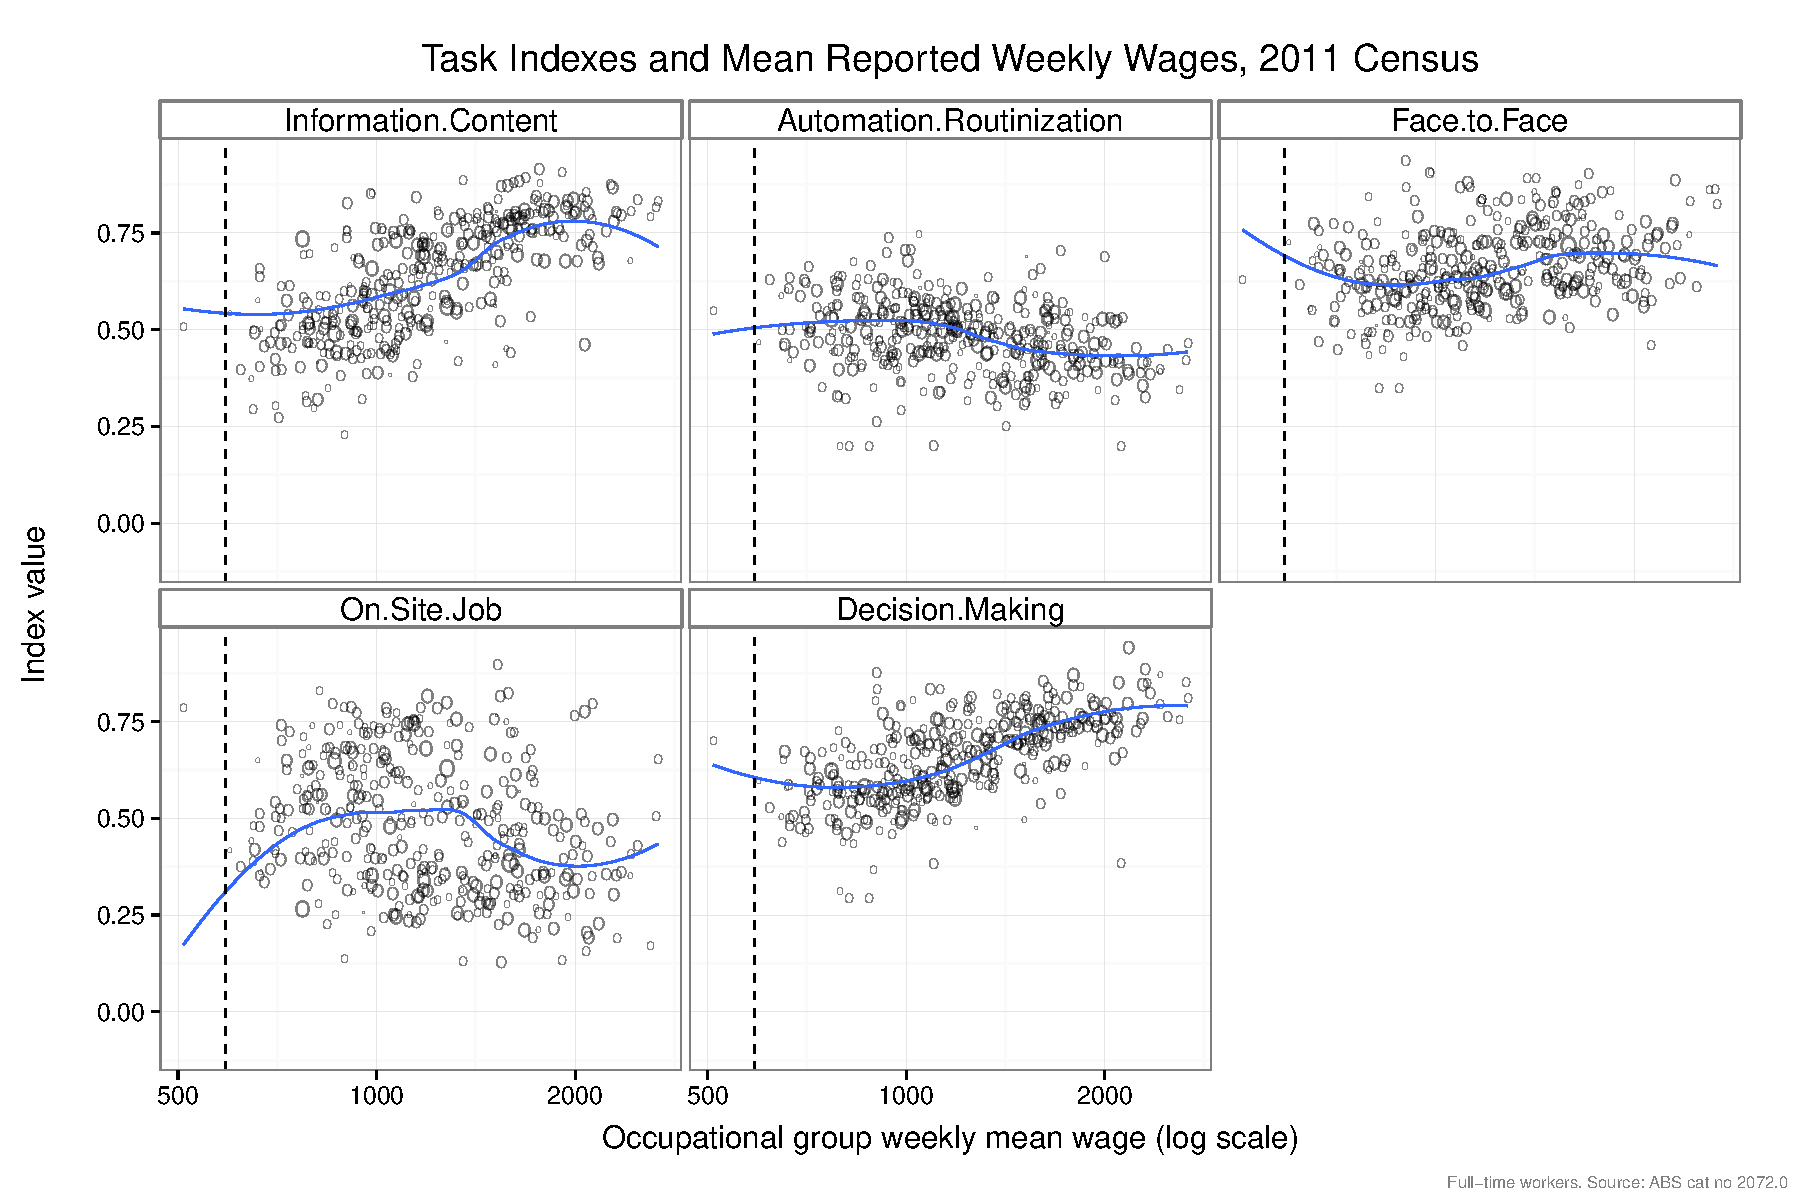
\includegraphics[width=\textwidth]{../figure/wages_indexes_4digit.pdf}
  \caption{Mean occupational weekly wage and task measure index values, at ANZSCO unit group (4-digit) level. The vertical dashed line is drawn at the level of the National Minimum Wage, of \$589.30 per week. Census respondents reporting full-time work are shown. The loess regression line is weighted by population; circle areas are proportional to population for each occupation. Notice that, when occupations are reduced to combined groupings, almost identical trends are observed (c.f. Figure~\ref{fig:meanocc2}). Sources: ABS cat 2072.0, O*NET, US Dept of Labor.}
  \label{fig:meanocc4dig}
\end{figure}

Two obvious patterns emerge in Figure~\ref{fig:meanocc4dig}: the information content and decision-making indexes are strongly positively related to conditional mean wages. These relationships are hardly surprising: professional and managerial work, which tends to be relatively highly remunerated, typically involves information processing and a greater degree of decision-making. Similarly, a negative relationship between automation/routinization and conditional mean wages is also evident. As \citet{Goos2009} argue, so-called `lovely' jobs, which are usually relatively well-paid, tend to involve primarily nonroutine activities, whereas lower-paid `middling' jobs tend to involve a greater proportion of repetitive activity. Finally, there does not appear to be a simple relationship between the face-to-face or on-site task indexes.

In order to test the routinization and outsourcing theories of occupational wage change, it is not enough to examine cross sections of the wage distribution at a given point in time. Rather, since our theory posits an increase in wage dispersion as a consequence of technical change, then these changes should be evident over a period of time. That there is a downward-sloping relationship between automation/routinization and conditional wages is insufficient: it must be demonstrated that this relationship is changing over time.

\section{A Simple Test of the Roy Model}\label{sec:direct}

In our simple industry-level analysis of different skill groups (\S\ref{sec:disappearing}), we concluded that it was the nature of jobs, rather than the level of `skill' they required, that mediated the impact of technical change. In this and the following analysis, we attempt to decompose changes in the wage distribution, according to the tasks involved in each job.

The key challenge to arise out of an exercise such as this is identification. As \citet{Fortin2011} point out, if panel data were available that included a longitudinal look at individuals who remained in a single occupation over a long period of time, and the data included a detailed breakdown of the tasks and skills required to do their jobs, then identification would be trivial. Instead, we have only repeated cross-sections of income data, and we must infer task data from occupational titles. 

Decomposition methods are especially powerful because they are able to extract relatively rich information from the data. However, this strength comes at the price of strong assumptions imposed on the data in order to guarantee parameter identification; the limitations these assumptions bring are shared by all decomposition methods, and are discussed in detail in section~\ref{sec:id}. The strength of these assumptions stem from the fact that decompositions provide only `shallow', empirical analyses of economic phenomena, and are not able to model `deep,' structural properties of the labor market. The most important of these restrictions, and possibly the least palatable, is the following. Despite motivating our model with Roy's model, a general-equilibrium framework, the empirical analysis presented below assumes that general equilibrium effects are completely dominated by first-order effects, so that market outcomes in each occupation's labor market depends only on the supply and demand for skills in that occupation.\footnote{Within a general equilibrium framework, this assumption is equivalent to the assumption of diagonal dominance \citep[p.233]{Arrow1971}.} This assumption is questionable: it is quite likely, for example, that a collapse in the demand for labor in one occupation, would cause some workers to change their occupational affiliations, triggering a shift in the supply of labor in other occupations. Nonetheless, this and other assumptions we employ below are standard in the inequality literature \citep[p.1]{Fortin2011}. These limitations will be discussed in greater detail, below.

\subsection{Model}

The desired decomposition is a relationship between occupations and their constituent tasks. Roy-type models posit that the wage an individual is paid depends on the skills demanded by that occupation, and the returns to the skills in question. One simple approach to identifying the contribution of each one of a worker's skills to the overall wage, considered by \citet{Firpo2011}, is to adapt the simple linearly additive functional form of \citet{Welch1969}. Welch assumed that an individual's wage is determined linearly by the individual skills that worker possessed.
\begin{assumption}[Linear additivity of returns to skills] \label{ass:linear}
  An individual $i$'s wage in occupation $j$ at time $t$ is set according to the sum of the returns $r_{jk}$ to skills $k$, $k=1,\dots,K$ required for that occupation:
\begin{equation}
  w_{ijt} = \theta_{jt} + \sum_{k=1}^K r_{jkt}S_{ik} + u_{ijt}, \label{eq:linear}
\end{equation}
Where $\theta_{jt}$ is a `base pay' term, $S_{ik}$ is an occupational skill level, and $u_{ijt}\sim i.i.d$ captures idiosyncratic characteristics of each worker. 
\end{assumption}

This is a strong assumption, which enjoys only limited empirical support. Linear additivity implies that the labor market in each occupation is free of general equilibrium effects arising from changes in other occupational wage structures.

Notice that in \eqref{eq:linear}, the returns to skill $k$ are particular to occupation $j$. This makes intuitive sense: since each individual is endowed with a particular mix of skills, which may not necessarily be useful in that individual's chosen occupation, there is no reason to expect the returns to certain skills to equilibrate across markets. In Roy's example described earlier, fly fishing skills of any level do not earn a return for workers engaged in rabbit hunting. % literature rejecting skill bundling

Following \citet{Firpo2011}, we perform two analyses of changes in the occupational wage. The first, outlined below, directly analyses the occupational wage profile as quantiles.

As a first step in the analysis, we directly analyze the relationship between occupational task measures and changes in the aggregate occupational wage profile. Under the maintained assumption that wages are linearly separable, it follows that changes in the occupational returns to a particular skill $r_{jk}$ will be observable in the aggregate wage profile.

Estimating a similar model of wage profiles, \citet{Juhn1993} suggested that, in regressions on occupational wage quantiles, a worker's rank within the wage distribution was a good proxy for that worker's ability. Thus, in aggregate, a fixed quantile effect $\lambda^q$ across groups could be interpreted as an aggregate measurement of changing returns to ability. We first estimate changes in the wage quantiles, for each occupation $j$ and each quantile $q$,
\begin{equation} 
  \Delta w_j^q = a_j + b_jw_{j0}^q + \lambda^q + \epsilon^q_j, \label{eq:quantiles}
\end{equation}
where $\lambda^q$ is an estimate of returns to skill at each quantile $q$. Under the maintained assumption that the returns to skill at each quantile of the wage distribution is independent of the actual occupation, then the parameters $a_j$ and $b_j$ describe the changes in each occupation over the study period.

The next step in the analysis is to decompose these changes according to the task we are interested in. These task measures, defined below, capture the ability to offshore or automate an occupation. Applying the first-step regressions defined above, we are now in a position to test the relationship between changes in occupational wage profiles and task indexes:
\begin{align}
  \hat{a}_j &= \gamma_0 + \sum_{h=1}^K\gamma_{jh}TC_{jh} + \mu_j, \label{eq:aeq} \\
  \hat{b}_j &= \delta_0 + \sum_{h=1}^K\delta_{jh}TC_{jh} + \nu_j. \label{eq:beq}
\end{align}

\subsection{Results}

The Roy model outlined above posits that, if the demand for labor of a particular type is shifting to the left, then two changes in the wage distribution should be visible: both mean wages and wage disperson should decrease. To test for these changes in the occupational wage distribution, we fit the model described above for two periods: from 1981/82 to 2011/12, using grouping I, and from 2000/01 to 2011/12, using grouping II. Once we have estimates of the change in mean and dispersion of the occupational wage distribution, we regress both of these measures against task measures for offshoring and routinization. Under the model hypothesized above, we therefore expect to obtain negative coefficient estimates for all five task measures.

Second-stage regression results for the periods 1981/82 to 2011/12 and 2000/01 to 2011/12 are tabulated in Tables~\ref{tab:quantreg1} and~\ref{tab:quantreg2}, respectively. In both tables, models 1---3 represent estimation results for \eqref{eq:aeq}, where the change in mean, $a_j^q$, is the dependent variable, and models 4---6 represent estimation results for regressions on the slope term $b_j^q$, specified in \eqref{eq:beq}. In models (1) and (4), coefficients associated with both outsourcing and routinizaton are entered together; whereas just outsourcing variables feature in models (2) and (5), and routinization variables in (3) and (6). Importantly, the sign and significance of the estimates in both tables are very similar, despite one dataset spanning 30 years, and the other a little over a decade. This suggests that occupational wage changes captured by the model are relatively recent. For the purposes of our discussion here, we will restrict our attention to Table~\ref{tab:quantreg2}, which covers the period 2000/01 to 2011/12. Note that while the sign of the coefficients can be interpreted, since these task measures were compiled from unit-free indexes and then arbitrarily normalized to have a unit range, the scale of the coefficients is aribitrary and has no direct interpretation. In particular, the reader is cautioned against comparing the magnitude of index coefficient estimates; it is not clear that this would be at all meaningful.

\documentclass{article}

\begin{document}

% Table created by stargazer v.4.5.1 by Marek Hlavac, Harvard University. E-mail: hlavac at fas.harvard.edu
% Date and time: Thu, Oct 10, 2013 - 12:36:34
\begin{table}[!htbp] \centering 
  \caption{Intercept and Slope of Change in Wage Quantiles, 1981/2 - 2011/12} 
  \label{} 
\begin{tabular}{@{\extracolsep{5pt}}lcccccc} 
\\[-1.8ex]\hline 
\hline \\[-1.8ex] 
 & \multicolumn{6}{c}{\textit{Dependent variable:}} \\ 
\cline{2-7} 
\\[-1.8ex] & \multicolumn{3}{c}{A (intercepts)} & \multicolumn{3}{c}{B (slopes)} \\ 
\\[-1.8ex] & (1) & (2) & (3) & (4) & (5) & (6)\\ 
\hline \\[-1.8ex] 
 Information.Content & 3.31 & $-$0.73 &  & $-$1.11 & 0.97 &  \\ 
  & (2.09) & (1.56) &  & (0.92) & (0.72) &  \\ 
  & & & & & & \\ 
 Automation.Routinization & $-$6.06 &  & $-$9.38$^{***}$ & 3.11$^{*}$ &  & 5.12$^{***}$ \\ 
  & (4.11) &  & (2.97) & (1.81) &  & (1.31) \\ 
  & & & & & & \\ 
 No.Face.to.Face & $-$0.01 & 1.39 &  & 0.26 & $-$0.48 &  \\ 
  & (2.96) & (2.29) &  & (1.30) & (1.05) &  \\ 
  & & & & & & \\ 
 No.On.Site.Work & 0.66 & 3.09$^{**}$ &  & $-$0.48 & $-$1.74$^{***}$ &  \\ 
  & (1.36) & (1.12) &  & (0.60) & (0.51) &  \\ 
  & & & & & & \\ 
 No.Decision.Making & 7.23$^{**}$ &  & 5.14$^{**}$ & $-$3.73$^{***}$ &  & $-$3.13$^{***}$ \\ 
  & (2.70) &  & (1.96) & (1.19) &  & (0.86) \\ 
  & & & & & & \\ 
 Constant & $-$1.35 & $-$0.97 & 3.46$^{***}$ & 0.39 & 0.19 & $-$1.68$^{***}$ \\ 
  & (1.85) & (1.52) & (1.05) & (0.81) & (0.70) & (0.46) \\ 
  & & & & & & \\ 
\hline \\[-1.8ex] 
Observations & 28 & 28 & 28 & 28 & 28 & 28 \\ 
R$^{2}$ & 0.50 & 0.33 & 0.29 & 0.57 & 0.38 & 0.40 \\ 
Adjusted R$^{2}$ & 0.38 & 0.25 & 0.23 & 0.48 & 0.30 & 0.35 \\ 
Residual Std. Error & 394.00 (df = 22) & 434.54 (df = 24) & 439.21 (df = 25) & 173.29 (df = 22) & 199.84 (df = 24) & 193.06 (df = 25) \\ 
F Statistic & 4.33$^{***}$ (df = 5; 22) & 3.96$^{**}$ (df = 3; 24) & 5.07$^{**}$ (df = 2; 25) & 5.90$^{***}$ (df = 5; 22) & 4.91$^{***}$ (df = 3; 24) & 8.25$^{***}$ (df = 2; 25) \\ 
\hline 
\hline \\[-1.8ex] 
\textit{Note:}  & \multicolumn{6}{r}{$^{*}$p$<$0.1; $^{**}$p$<$0.05; $^{***}$p$<$0.01} \\ 
 & \multicolumn{6}{r}{Occupational grouping #1 used, with 28 occupational groups.} \\ 
\normalsize 
\end{tabular} 
\end{table} 
\end{document}





% Table created by stargazer v.4.5.1 by Marek Hlavac, Harvard University. E-mail: hlavac at fas.harvard.edu
% Date and time: Fri, Oct 11, 2013 - 23:16:58
\begin{sidewaystable}[!htbp] \centering 
  \caption{Intercept and Slope of Change in Wage Quantiles, 2000/01 - 2011/12} 
  \label{} 
\begin{tabular}{@{\extracolsep{0pt}}lcccccc} 
\\[-1.8ex]\hline 
\hline \\[-1.8ex] 
 & \multicolumn{6}{c}{\textit{Dependent variable:}} \\ 
\cline{2-7} 
\\[-1.8ex] & \multicolumn{3}{c}{A (intercepts)} & \multicolumn{3}{c}{B (slopes)} \\ 
\\[-1.8ex] & (1) & (2) & (3) & (4) & (5) & (6)\\ 
\hline \\[-1.8ex] 
 Information content & $-$6.20 & $-$8.77$^{***}$ &  & 0.97 & 1.48$^{***}$ &  \\ 
  & (4.07) & (3.11) &  & (0.60) & (0.46) &  \\ 
  & & & & & & \\ 
 Automation/routinization & $-$8.22 &  & $-$17.16$^{***}$ & 1.14 &  & 2.58$^{***}$ \\ 
  & (8.60) &  & (6.04) & (1.27) &  & (0.89) \\ 
  & & & & & & \\ 
 No face-to-face contact & 3.72 & 2.33 &  & $-$0.41 & $-$0.41 &  \\ 
  & (6.14) & (4.00) &  & (0.90) & (0.60) &  \\ 
  & & & & & & \\ 
 No on-site work & 7.14$^{**}$ & 8.87$^{***}$ &  & $-$1.06$^{**}$ & $-$1.38$^{***}$ &  \\ 
  & (2.58) & (2.03) &  & (0.38) & (0.30) &  \\ 
  & & & & & & \\ 
 No decision-making & 5.39 &  & 12.92$^{***}$ & $-$1.02 &  & $-$2.16$^{***}$ \\ 
  & (5.05) &  & (4.09) & (0.74) &  & (0.60) \\ 
  & & & & & & \\ 
\hline \\[-1.8ex] 
Observations & 29 & 29 & 29 & 29 & 29 & 29 \\ 
R$^{2}$ & 0.48 & 0.44 & 0.29 & 0.51 & 0.47 & 0.34 \\ 
Adjusted R$^{2}$ & 0.36 & 0.38 & 0.24 & 0.40 & 0.40 & 0.29 \\ 
Residual Std. Error & 15.43 (23) & 15.23 (25) & 16.85 (26) & 2.27 (23) & 2.27 (25) & 2.48 (26) \\ 
F Statistic & 4.18$^{***}$ (5; 23) & 6.67$^{***}$ (3; 25) & 5.40$^{**}$ (2; 26) & 4.73$^{***}$ (5; 23) & 7.26$^{***}$ (3; 25) & 6.59$^{***}$ (2; 26) \\ 
\hline 
\hline \\[-1.8ex] 
\textit{Note:}  & \multicolumn{6}{r}{$^{*}$p$<$0.1; $^{**}$p$<$0.05; $^{***}$p$<$0.01} \\ 
 & \multicolumn{6}{r}{Occupational grouping 2 used, with 29 occupational groups.} \\ 
\normalsize 
\end{tabular} 
\end{sidewaystable} 



Table~\ref{tab:quantreg1} does not present any strong evidence for the routinization hypothesis, but it does suggest some interesting evidence for the outsourcing hypothesis. Estimates for variables thought to be associated with routinization, information content and automation/routinization, are shown in columns (3) and (6). They do not appear to have a consistent effect across the income distribution, and the coefficient estimates are not significantly different from zero. We therefore exclude these variables from further consideration from our model.

The evidence for the routinization and outsourcing theories presented in Table~\ref{tab:quantreg1} is somewhat mixed. As expected, a higher level of routinization in an occupation is associated with a decrease in wages, across all quantiles of the wage distribution. However, automation is also associated with {\em greater} wage dispersion, not less. Consistent with the theory, the slope terms for `no on-site work' and `no decision-making' are both signficiantly negative, so that offsite work and a lack of decision-making are both associated with a decreased dispersion of wages. However, contrary to the theory, estimates for changes in the mean wage are significantly {\em positive}, the opposite of the sign predicted by the theory. Similarly, the evidence for `information content' is conflicting: although we expect both the change in mean and dispersion to be negative, the change in dispersion is in fact significantly positive.

\subsection{Discussion}

The results in Table~\ref{tab:quantreg1} stand in contrast to \citet{Firpo2011}, who found that, in the United States between 1988 and 2002, three out of the five indexes given here are associated with negative changes in both the mean and dispersion of wages. Indeed the mixed results discussed above suggest a number of possible explanations. First, it is possible that the proposed Roy model is inadequate, and simply does not explain changes in occupational wage profiles. Second, changes in the wage profile may not be uniform across the earnings spectrum, as \eqref{eq:quantiles} assumes. Finally, it could be that these results are simply an artefact of the occupational mapping or aggregation scheme employed, or structural differences between the United States and Australian labor market.

One major difference with the US labor market that could explain the unexpected increase in these jobs, is the presence of a sizeable minimum wage in Australia. In Figure~\ref{fig:meanocc4dig}, notice that the 2011 National Minimum Wage of \$622.30 per week, illustrated by the dashed line, is quite close to the conditional mean wage of some occupations. It is therefore possible that, at some wage levels, changes in the mean or dispersion of wages have very little to do with the properties of the job, but instead are due to institutional factors. Proximity of the wage distribution to the level of the minimum wage suggests that the presence of non-linearities in the relationship between tasks and wages could be important.\footnote{The results presented in Tables~\ref{tab:quantreg1}~and~\ref{tab:quantreg2} are robust to the exclusion of subsets of quantiles. In particular, excluding quantiles close to the minimum wage has negligible effect on parameter estimates.}

\section{Decomposing Wage Changes}

In this final stage of the analysis, we attempt to examine the evidence for a causal link between changes in technology and changes in the wage distribution. First, we use the approach suggested by \citet{DiNardo1996} to perform an aggregate decomposition of wages, separating changes in the wage distribution into a composition effect and a wage structure effect. We then proceed one step further, and attempt to explain the wage structure effect by our technology indexes.

\subsection{Aggregate Decomposition} \label{sec:id}

The theoretical approach we follow here is sketched in the previous chapter (\S\ref{sec:reweight}), and described in detail in \citet{DiNardo1996}. Recall that, the goal of decomposition approaches is to separate changes in the wage distribution into two parts:
$$
\Delta_O = \Delta_S + \Delta_X,
$$
where $\Delta_X$ is the composition effect, and $\Delta_S$ is the wage structure effect. The composition effect is that part of the wage distribution explained by changes in human capital and demographic variables such as potential experience and educational attainment. The wage structure effect is that part which remains unexplained, and which we assume can be explained by our derived task indexes.

However, before we can proceed with estimation, we must impose further assumptions on our data. First, we require that the support of covariates $X$ is the same for both time periods. In other words, it should not be possible to unambiguously predict which time period an observation belongs to, simply by observing the value of its covariates. 
\begin{assumption}[Overlapping support] \label{ass:overlap}
  Let the support of wage setting factors in both periods $[X',\epsilon']'$ be $\mathcal{X}\times\mathcal{E}$. For all $[x',e']' \in \mathcal{X}\times\mathcal{E}$,  $0 < \Pr[T=0 | X=x, \epsilon=e] < 1$.
\end{assumption}
Importantly, Assumption~\ref{ass:overlap} means that the set of occupational titles in both periods must be the same, even though many new types of occupational titles have been created since 1981/82. However, although there might have been large changes within occupational groups, a counterpart for each ANZSCO minor group was readily identified in the 1981/82 classification.

Further, in order to identify the explained and unexplained effects of the covariates, we require that the error term $\epsilon$ has the same conditional distribution in both time periods. This is known as the {\em ignorability} assumption.
\begin{assumption}[Ignorability]
  For $T\in\{0,1\}$, let $(T, X, \epsilon)$ have a joint distribution. Then, for all $x\in \mathcal{X}$, $\epsilon$ is independent of $T$ given $X=x$.
\end{assumption}

The above assumptions imply at least one fact that is clearly false: that occupational titles in the first period have the same meaning as occupations in the last period. Although it can be argued that, say, the occupation of 'Lawyer' is largely unchanged between the 1980s and the 2000s, the same cannot be said for certain technical professions. The activities of a `Surveyor,' for example, has been greatly altered by the introduction of GPS technology and portable computers. However, this problem is mitigated somewhat by aggregating occupations into larger groups; see \citet{Firpo2011} for a discussion.

\subsubsection{Results}

Figure~\ref{fig:aggregate} plots results for the aggregate wage decomposition across the wage distribution for the same two comparison periods as before, 1981/82--2009/10 and 2000/01--2009/10. The blue lines indicate overall changes in the log wage distribution over the time period, and bear the familiar `banana' shape seen in Figure~\ref{fig:banana} (although these charts are not disaggregated by sex.)\footnote{Figure~\ref{fig:aggregate} is weighted to match the 1981/82 covariate distribution, whereas Figure~\ref{fig:banana} is weighted to match  2009/10. Consequently, the charts will not have exactly the same profile.} The green line plots the composition effect, which arises from changes explainable by the work force's observable human capital attributes. And finally, the red line plots the difference between these lines, the wage structure effect, which we attribute to changes in the technological environment over the period.

\begin{figure}
  \centering
  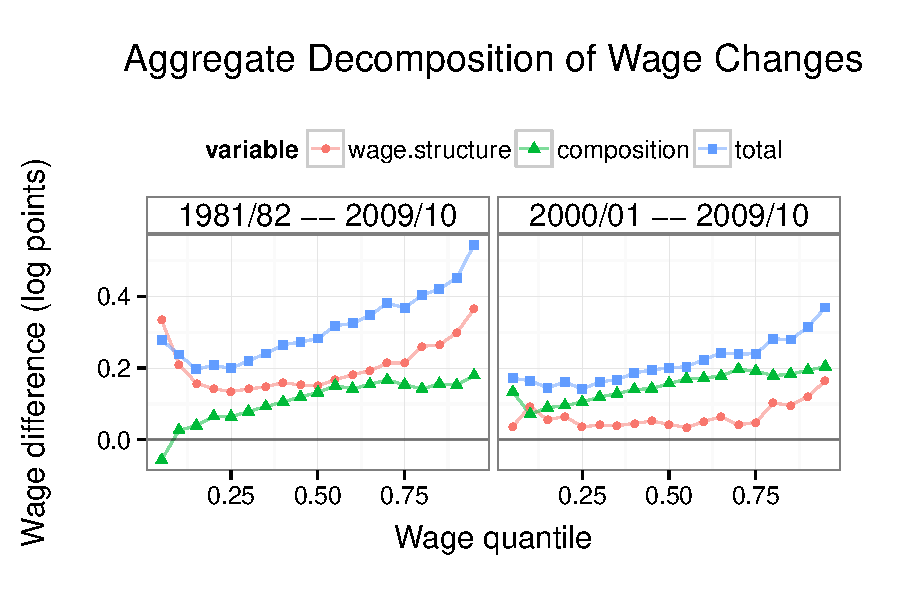
\includegraphics[width=\textwidth]{../figure/aggregate_decomp.pdf}
  \caption{Aggregate decomposition of wage changes, 1981/82--2011/12 and 2000/01--2001/12. Sources: ABS SIH 1981/82, 2000/01, 2011/12; ABS cat. no. 6401.0, 1220.0, 1223.0, 1288.0.; US Dept of Labor.}
  \label{fig:aggregate}
\end{figure}

The left-hand panel spans a period of about 30 years, while the right-hand panel spans just one decade. As expected, wage changes are larger for the 30-year timespan than they are for the shorter period. However, for the longer period, notice that it is the wage structure effect that dominates, whereas between 2000/01 and 2009/10, the composition effect dominates. This suggests that, consistent with findings from studies in the United States and Europe, the technological impact on the wage distribution occured mainly in the 1980s and 1990s.

Notice also that, for the most part, the curves are upward-sloping, especially in the upper three-quarters of the wage distribution. This is consistent with the theories of technical change we have discussed so far, which posit that more `skilled' workers (here proxied by their position in the wage distribution), benefit more from technical change. However, notice the U-shaped wage structure curve in the left-hand panel: there were significantly greater gains in the lower quartile of the wage distribution than there were in the middle two quartiles. This is a puzzle: perhaps there are other factors that are systematically influencing low-income jobs.\footnote{There are many possible explanations for this effect. Since 1981/82, the national minimum wage was introduced. Further, in this study we do not have data on union membership, which has been shown to explain a great deal of changes in the wage distribution \citep{Leigh2013,Borland1996}.}

\subsection{Detailed Wage Structure Decomposition}

In order to test the routinization and outsourcing hypothesis, we wish to decompose the wage structure component into contributions from our occupational task indexes. The assumptions stated so far, although sufficient for identifying the wage structure component ($\hat{\Delta}_S$) and endowment effect component ($\hat{\Delta}_X$) of the aggregate decomposition, are insufficient to identify the components of the wage structure.

\citet[p.27]{Fortin2011} show that non-parametric estimates of the detailed decomposition require assumptions that cannot be maintained in this context. For example, the `independence' condition, found in \citet{Matzkin2003}, must hold:
\begin{assumption}[Independence]\label{ass:indep}
  For $T\in\{0,1\}$, $X$ is uncorrelated with $\epsilon$ in time $T$.
\end{assumption}
Most decompositions of the determinants of wages, including this one, follow the Mincerean `human capital' approach, which suggests that the primary determinants of wages are investments in education and experience, which enhance productivity \citep{Mincer1962}. For that reason, these covariates are included in $X$ in this study. However, as is well-known, OLS regression estimates of Mincer-style wage equations tend to exhibit endogeneity bias, since observable characteristics (such as years of schooling) tend to be correlated with unobserved characteristics such as general ability or talent \citep{Card1999}. Consequently, any regression specification that omits an accurate measure of `ability' will exhibit endogeneity bias, since the omitted variable will cause explanatory variables such as schooling to be correlated with the error term. That is to say, the independence property is violated.

However, the impracticality of Assumption~\ref{ass:indep} can be avoided by imposing the linear functional form in Assumption~\ref{ass:linear} \citep[p.28]{Fortin2011}. Furthermore, the linear functional form assumption allows for heteroskedasticity. In this application, this is a useful property, since income variance increases with educational attainment.

The choice of base case for the detailed decomposition is non-trivial. After experimenting with a number of options, male high school graduates with 15-20 years of potential experience were found to be the base case that yielded the most stable results.

\subsubsection{Results}

Detailed decomposition results for the wage structure effect, according to our task measure indexes, are shown in Figure~\ref{fig:structure}.\footnote{Our detailed decomposition also accounts for potential experience (8 dummies), educational attainment (five dummies), marital status and sex. These variables are not reported.} The chart shows impact a unit change in each variable would have on the log wage, {\em ceteris paribus}, at quantiles across the wage distribution. A plotted value of zero indicates `no change'. Points above the x-axis indicate that task measure explains an increase in wage at that quantile, and vice-versa for points below the x-axis.

\begin{figure}[th]
  \centering
  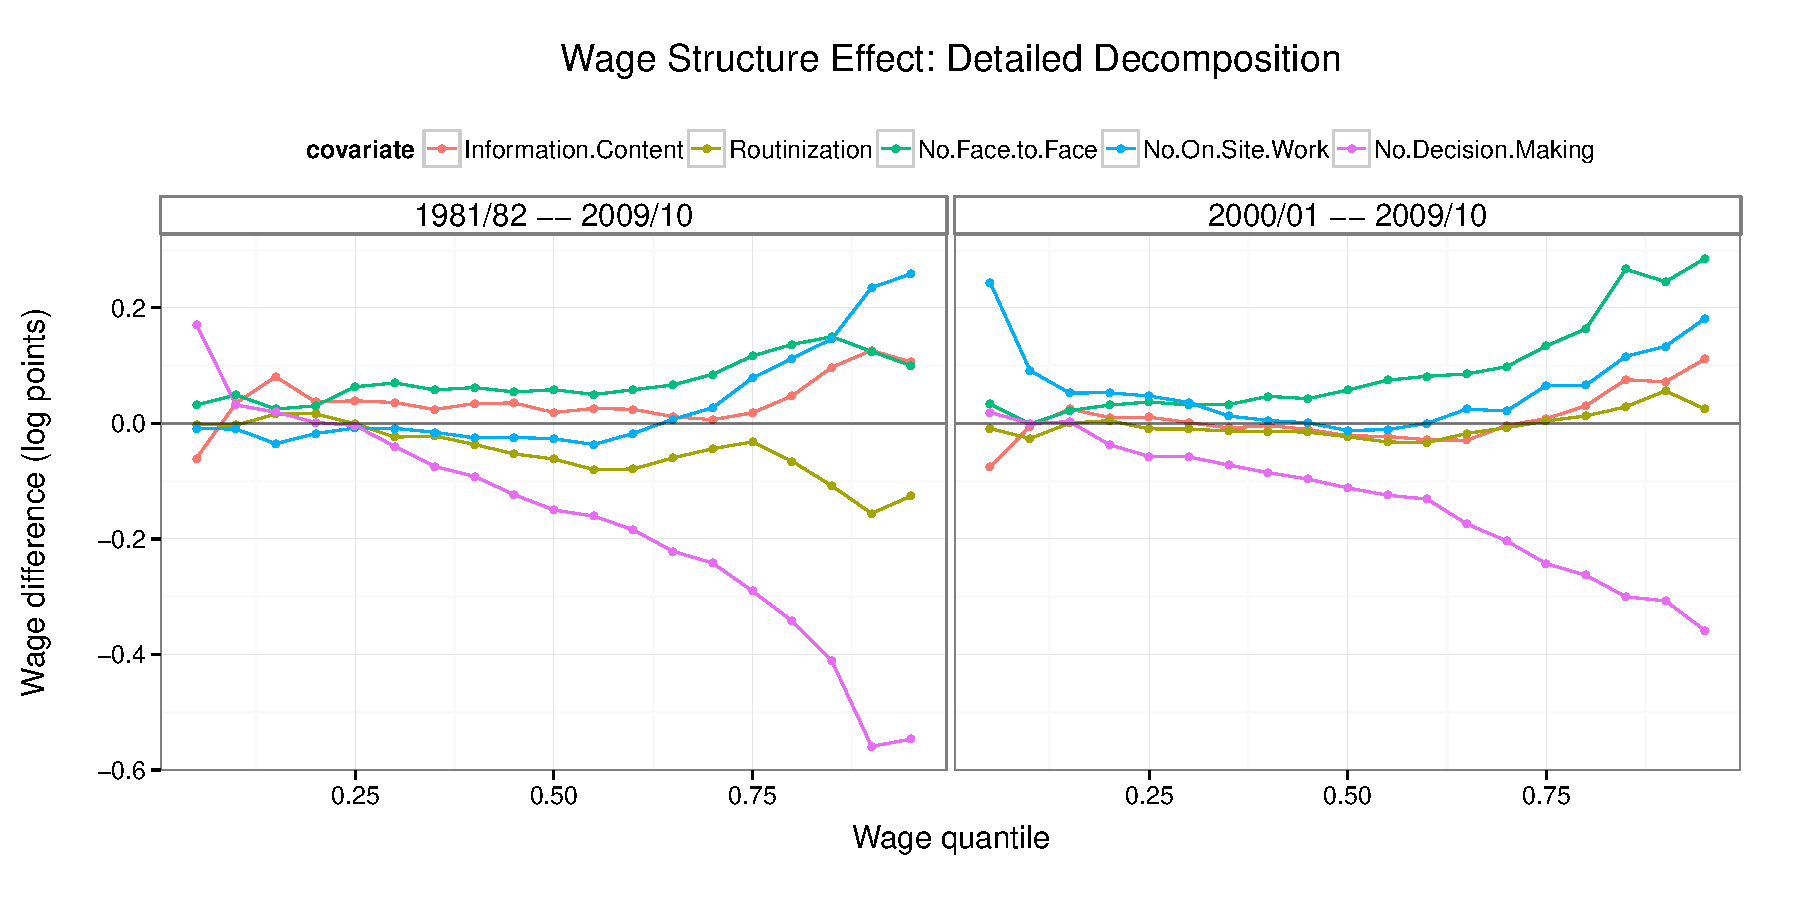
\includegraphics[width=\textwidth]{../figure/structure_decomp.pdf}
  \caption{Detailed structural decomposition of wage changes, 1981/82--2011/12 and 2000/01--20011/12. Note that, as before, since task indexes are unit-free, direct comparisons between magnitudes of index coefficients is not meaningful. Following \citet{Firpo2011}, decomposition charts are presented without confidence intervals. Sources: ABS SIH 1981/82, 2000/01, 2011/12; ABS cat. no. 6401.0, 1220.0, 1223.0, 1288.0.; US Dept of Labor.}
  \label{fig:structure}
\end{figure}

The decomposition shown in Figure~\ref{fig:structure} demonstrates an important point: the impact of task measures are non-uniform across the skill spectrum. In particular, the impact of decision making is highly variable, depending on the wage quantile. Consider the non-decision-making index in the 1981/82--2009/10 panel. In the 5th percentile, the absence of decision-making is associated with an increase in wages, but a decrease in wages between the 25th and 95th percentiles. Notice that the trend for the (lack of) decision-making variable is very similar in both the 1981/82--2009/10 and 2000/01--2009/10 charts. This suggests that the structural changes that led to the increasing value of management roles for high-income earners occurred over the period of the 2000s.

Figure~\ref{fig:structure} provides evidence for the routinzation hypothesis, but only in the top half of the income distribution. Jobs that involve routine tasks are associated with a negative change in wages between 1981/82 and 2009/10. However, this trend is not present in the most recent decade, suggesting that replacement of routine jobs occurred in the 1980s and 1990s. This is consistent with the findings of \citet{Firpo2011}, who find a negative routinzation effect only in the 1980s.

Interpretation of the other variables is somewhat more difficult. In particular, remuneration for jobs with no face-to-face content and an absence of on-site work appears to have grown for higher wage quantiles. These variables, which were included in order to test the `offshoring' hypothesis, could instead be detecting the rise remuneration for information-economy jobs experienced in the 1990s and 2000s. Although it is true that call center operators do not have to be on a client's site or see them face-to-face in order to do their jobs, the same can be said for a computer programmer, an occupation for which remuneration grew dramatically over the 1990s and 2000s. Indeed, at top wage percentiles, a higher information content is also associated with higher earnings, which does lend weight to this explanation.

\section{Conclusions}

In this chapter, we brought some of the models we considered here to the Australian data. Contrary to the experience of foreign labor markets, but consistent with older Australian studies, we found that the widening income distribution does not appear to being driven by a widening `college premium,' which casts doubt on the `canonical' model of SBTC.

We did, however, find support for the theory that the wage share of middle-skill jobs is declining. Consistent with other studies in foreign labor markets, this could be suggestive of firms investing in plant equipment in order to replace certain types of workers. However, this evidence is extremely weak, and can only be treated as a correlation.

Direct tests on the wage structure suggested that there was no simple relationship between the constructed task indexes and the wage structure. Although the change in the dispersion of `off-shoreable' jobs was significant and in the expected direction for two out of three of the indexes, changes in base wages were generally positive. While it is possible that the minimum wage or other institutional factors rendered this model inappropriate, these results nonetheless demonstrate that the relationship between tasks and wage changes is complex.

Decomposition results suggest that the bulk of structural changes in the wage distribution occurred in the 1980s and 1990s, with wage changes in the 2000s being mostly accounted for by changes in individuals' wage-related variables such as educational attainment and experience.

After eliminating the change that {\em is} explainable by human capital variables, some evidence for the routinization hypothesis remained: for individuals in the upper three quarters of the wage distribution, routine work was associated with a lower wage in 2009/10 than in 1981/82. However, this structural change appears to have taken place in the 1980s and 1990s, not the 2000s. In the 2000s, we found evidence of the rising value of management tasks in a job, the magnitude of which grows across the income distribution. 

%%% Local Variables: 
%%% mode: latex
%%% TeX-master: "paper"
%%% End: 
